\documentclass{beamer}
\usepackage{beamerthemesplit}
\usepackage{lmodern}
\usepackage{graphicx} 
\usepackage[absolute,overlay]{textpos}
\usepackage{hyperref}
\usepackage{epstopdf}

\setbeamercolor{framesource}{fg=black}
\setbeamerfont{framesource}{size=\tiny}

\newcommand{\source}[1]{\begin{textblock*}{4cm}(8.5cm,8.1cm)
	\begin{beamercolorbox}[ht=0.5cm,right]{framesource}
		\usebeamerfont{framesource}\usebeamercolor[fg]{framesource} Source: {#1}
	\end{beamercolorbox}
\end{textblock*}}


\title{Evacuation Bottleneck}
\subtitle{Simulating a Panic on a Cruise Ship}
\author{Johannes Weinbuch, Benedek Vartok}
\date{\today}

\begin{document}
\frame{\titlepage}

%Johannes
\begin{frame}
	\frametitle{Outline}
	\tableofcontents
\end{frame}

\section{Introduction}

%Johannes
\begin{frame}
	\frametitle{Our Research Object}
	\begin{columns}
		\begin{column}{5cm}
			\begin{itemize}
				\item Costa Voyager
				\item Capacity: 836 passengers
				\item 8 Rescue Boats
				\item In distress at sea in 2005
			\end{itemize}
		\end{column}
		\begin{column}{5cm}
			\begin{centering}
				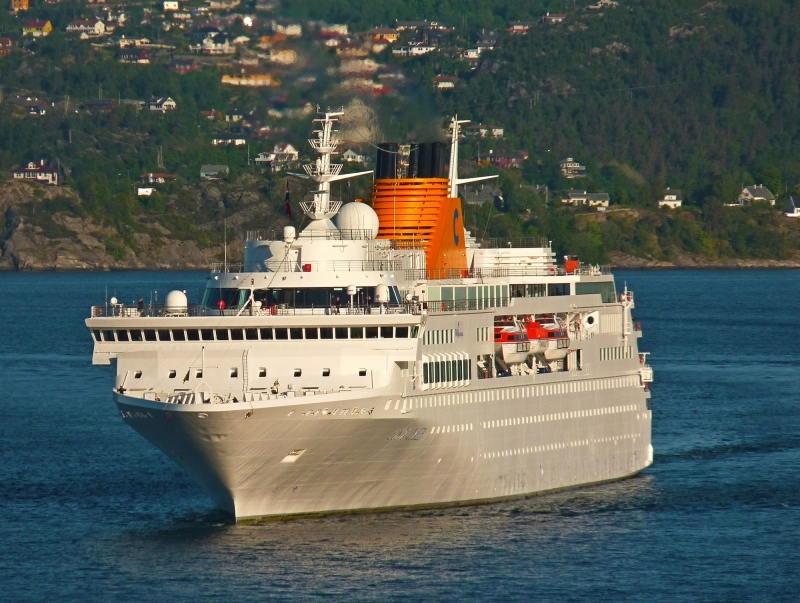
\includegraphics[scale=0.5]{images/costavoyager.jpg}
			\end{centering}
		\end{column}
	\end{columns}
	\source{http://www.shipspotting.com, Picture taken by Roy Batty}
\end{frame}

%Benedek
\section{Models and Implementation}

\subsection{Program Structure}
\begin{frame}
	\frametitle{Program Structure}
	\begin{enumerate}
		\item Load configuration
			% initialization from file
		\item Loop over simulation steps
			% depending on timestep and maximum duration
		\begin{enumerate}
			\item Place new agents
				% in spawn zones, if there are any left
			\item Handle filled exits
				% when agents fill up a rescue boat
			\item Progress agents with calculated forces
			\item Remove exited agents
				% when agent reaches boat, he leaves simulation
			\item Plot current state (optional)
				% show layout with agents
		\end{enumerate}
		\item Plot and save final data
			% show time series of rescue boat occupations
	\end{enumerate}
	% in the following slides we will go into
	% the more interesting points in detail
\end{frame}

%Johannes
\subsection{Input, Configuration}
\begin{frame}
	\frametitle{The Deck Plan}
	\begin{columns}
		\begin{column}{5cm}
			\begin{itemize}
				\item Colormap
					\begin{itemize}
						\item Allows any number of zones
					\end{itemize}
				\item Scaling
				\item Greatly simplyfied
			\end{itemize}
		\end{column}
		\begin{column}{2.5cm}
			\begin{center}
				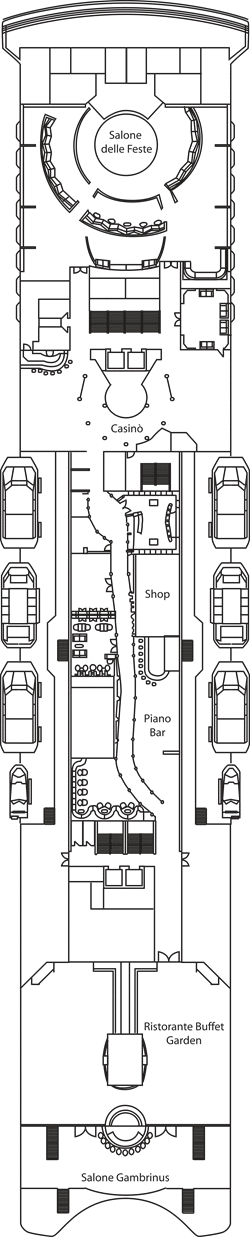
\includegraphics[height=5cm]{images/deckbefore.png}
			\end{center}
		\end{column}
		\begin{column}{2.5cm}
			\begin{center}
				
\includegraphics[height=5cm]{images/deckafter.png}
			\end{center}
		\end{column}
	\end{columns}
	\source{http://www.kreuzfahrtberater.de}
\end{frame}

%Benedek
\begin{frame}
	\frametitle{Configuration File}
	\begin{itemize}
		\item Simulation parameters intialized from a file:
			\begin{itemize}
				\item Deck configuration
					% deck image file to use, pixel_per_meter setting (scale);
					% number of spawning and exiting zones,
					% number of agents to spawn and exit capacities
				\item Plotting options
					% whether to store frames
				\item Physical and behavioral parameters
					% of simulation and agents, such as time-step and
					% panic level
			\end{itemize}
		\item Simple syntax makes automated generation easy
			% to sweep over a range of parameters
	\end{itemize}
\end{frame}

%Benedek
\subsection{Placement of New Agents}
\begin{frame}
	\frametitle{Placement of New Agents}
	\begin{itemize}
		\item Spawning zones as entering areas for agents
			% each with a given number of total agents to spawn
		\item In each step, remaining agents are tried to be placed
		\item If spawning zones are too full, new agents can only appear in later steps
		\item Nice model for steady inflow of agents
			% e.g. stairs, agents coming from different floor
	\end{itemize}
\end{frame}

%Benedek
\subsection{Filled Exits}
\begin{frame}
	\frametitle{Filled Exits}
	\begin{itemize}
		\item Rescue boats modeled with limited capacities
		\item If a boat gets full, agents need to be informed
		\item Two implementation approaches:
			\begin{itemize}
				\item Instantaneous update
					% every agent knows about the closed exit immediately
					% and updates his desired path accordingly
				\item Gradual circle-shaped spreading of information
					% modelling slow communication between agents;
					% new information starts spreading from the exit zone
					% outwards
			\end{itemize}
	\end{itemize}
\end{frame}

%Benedek
\subsection{Forces}
	% physical simlulation in continous space ==> Newtonian model with forces
\begin{frame}
	\frametitle{Forces}
	\begin{itemize}
		\item As described in Helbing's paper \mbox{``Simulating dynamical features
		      of escape panic''}
		\item Three main forces act on agents:
			\begin{itemize}
				\item Desired direction
					% agents try to achieve a velocity vector pointing in
					% the direction of the nearest open exit
				\item Repulsion \& friction between agents
					% they don't want to get too close to each other,
					% "social force";
					% if they touch, they need to be separated physically and
					% some friction appears
				\item Repulsion \& friction from walls
					% same as other agents, walls are avoided
			\end{itemize}
		\item Motions calculated with Leap-Frog integration method
			% with the forces known, agent motions are integrated with Leap-Frog
	\end{itemize}

	% TODO: sketch
\end{frame}

% TODO (not all):
%       - restructure Model/Implementation in presentation
%       - code reuse
%       - main loop
%       - spawning new agents
%       - removing exited agents
%       - proceeding agents
%       - updating desired vector fields
%       - plotting

%Benedek

%Johannes
\section{Results}

\subsection{Passenger Distribution}
\begin{frame}
	\frametitle{Distribution of the Agents to the Exits}
	\begin{itemize}
		\item The distribution depends strongly on the geometry of the ship.
		\item There was no case where the agents really distributed over the exits
		\begin{itemize}
			\item Weakness in the model
			\item More realistic: go for the shortest individual evacuation time
		\end{itemize}
		\item realistic update for propagation of information
		\item Video
	\end{itemize}
\end{frame}


\subsection{Panic Level}
\begin{frame}
	\frametitle{Effect of desired speed to the overall evacuation time}
	\begin{columns}
		\begin{column}{5cm}
			\begin{itemize}
				\item We could reproduce the results from Helbing, Farkas and Vicsek for low panic levels
				\item High panic levels: problem!
			\end{itemize}
		\end{column}
		\begin{column}{5cm}
			\begin{figure}
				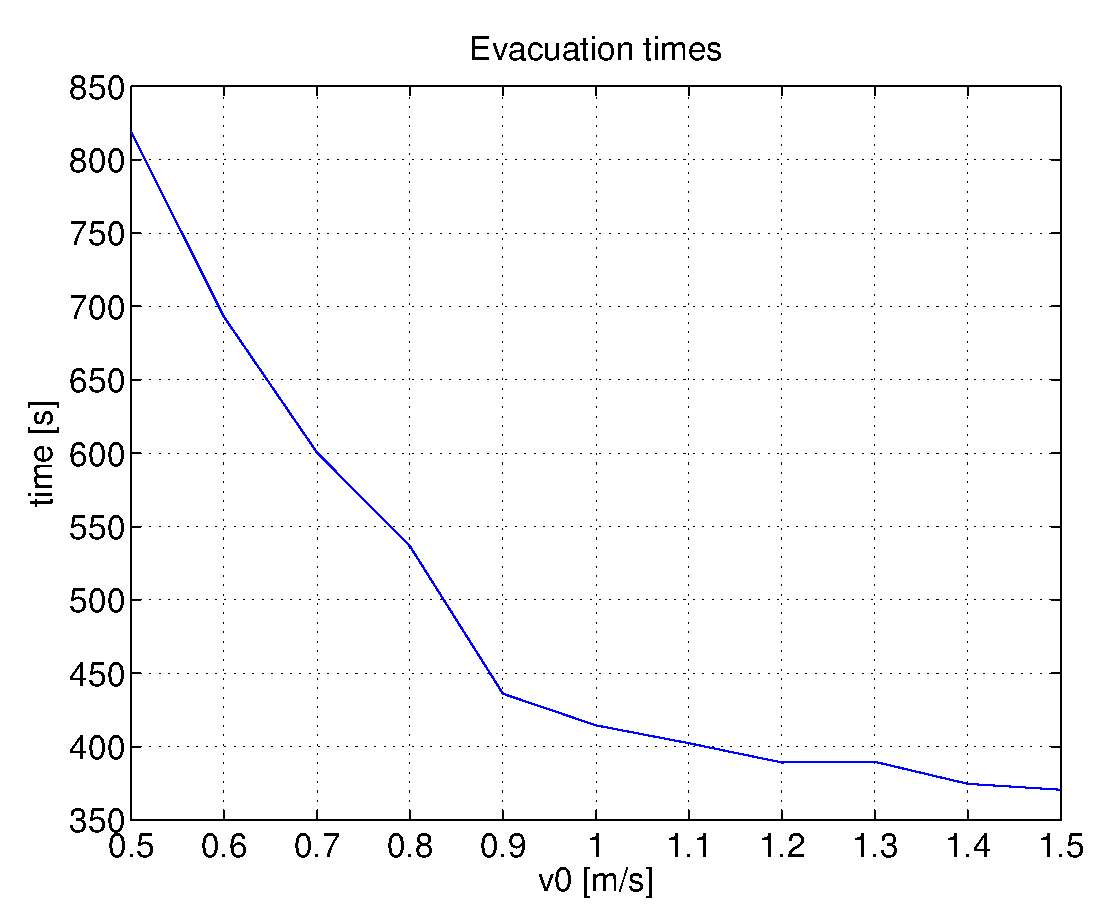
\includegraphics[width=5cm]{images/evactimes1to11.eps}
			\end{figure}
		\end{column}
	\end{columns}
\end{frame}

\subsection{Outtakes}

\begin{frame}
	\frametitle{All the things you don't want to happen}
	\begin{itemize}
		\item Agents were stuck in Walls
		\begin{itemize}
			\item Even the tiniest timesteps didn't help
		\end{itemize}
		\item MATLAB does not behave as expected in batch mode
		\begin{itemize}
			\item Simulation works in foreground, crashes in background
			\item No error message, just silently writing crashdumps to home
		\end{itemize}
		\item No reproducability even with fixed random seed in our group
		\begin{itemize}
			\item Different versions of MATLAB
		\end{itemize}
	\end{itemize}
\end{frame}


\section{Summary and Outlook}
\begin{frame}
	\frametitle{Some points to take away}
	\begin{itemize}
		\item The basic results could be reproduced
		\item The model is not very well suited for multiple exits
		\begin{itemize}
			\item There should be a heuristic to decide for a direction
		\end{itemize}
		\item Use the power of Open Source Software (OSS)!
	\end{itemize}
\end{frame}

\begin{frame}
	\frametitle{You ask -- We answer}
	\begin{itemize}
		\item Now it's your turn
	\end{itemize}
\end{frame}

\end{document}
